\documentclass[fontsize = 12pt]{scrartcl}

% Encoding of documents
	\usepackage[utf8]{inputenc}
	\inputencoding{utf8}
	\usepackage[T1]{fontenc}

% Silbensetzung und Automatisch Anpassung der Sprache in generierten Inhalten
	\usepackage[english]{babel}
	

% Mathematical character set 
	\usepackage{amsmath,amssymb,amstext}
 	
% Hyperef
	\usepackage{hyperref}

% Font
	\usepackage{txfonts} % TimesNewRoman als Shrift des Fließtextes
					     % Helvetica als serifenlose Schrift für Beispielsweise Überschrift 		
    % \usepackage{pxfonts}
	% \usepackage{lmodern}

	%\usepackage{setspace} % zum Einstellen des zeilenabstandes
	%\setstretch{1.00}

	% Tabular and figure caption
	\usepackage[nooneline]{caption} % noonline sorgt dafür das beschriftung linksbündig ist
	%More info:  https://www.namsu.de/Extra/pakete/Caption.html	
    %	\captionsetup[figure]{labelfont=it, textfont=it} % figure captions
	%   \captionsetup[table]{labelfont=bf, textfont=it} % tabular captions


% Einführen von Bildern
\usepackage{rotating} % Einfügen und rotieren von Bildern und Graphiken
% \usepackage[final]{graphicx} % Einfügen von Bildern
						     % Setze das Optionale Argument zu 'draft' für schnelleres komplilieren
						     % dann werden bilder durch Rahmen ersetzt.
\usepackage{subcaption}
\usepackage{wrapfig}         % bilder im Fließtext

% Utils
\usepackage{braket}
\usepackage{autonum}
\usepackage{tikz}

% Makro-commands
\newcommand{\corr}[1]{\left\langle #1 \right\rangle}
\newcommand{\Sp}[1]{\textit{Sp}\left( #1 \right)}
\renewcommand{\exp}[1]{\textit{exp}\left( #1 \right)}
\newcommand{\tlim}{ \underset{V,N \to \infty}{\text{lim}^{*}}}

% Umgebungs-commands
\usepackage{mdframed}
\newmdenv[backgroundcolor=black!5, skipabove=12pt, linecolor=white, innerbottommargin = 10pt,
frametitlerule=true, frametitlerulecolor=black, frametitlebackgroundcolor=black!10, frametitlerulewidth=0pt]{grayframe}


%tikz commands
\usetikzlibrary{positioning}
\usetikzlibrary{shapes}
\usetikzlibrary{arrows}
\usetikzlibrary{decorations.markings}

\tikzset{
  arrow_outer/.style={-latex, shorten >=5, shorten <=5,  very thick, color = blue!80}, 
  arrow_inner/.style={-latex, shorten >=2, shorten <=2, thick, color = blue!80},
  arrow_start/.style={-latex, shorten >=2, shorten <=2, thick, color = black!80},
  arrow_double/.style={<->, shorten >=2, shorten <=2, very thick, color = black!80},
  arrow_down/.style={->, shorten >=2, shorten <=2, very thick, color = black!80},
  arrow_grid_in/.style={-latex, shorten >=2, shorten <=2, ultra thick, color = black!100},
  arrow_grid_out/.style={-latex, shorten >=2, shorten <=2, ultra thick, color = black!50},
  grid_point/.style={circle, draw, color=black!100, fill=black!100, minimum size = 8pt, inner sep = 0},
  small_grid_point/.style={circle, draw, color=black!100, fill=black!100, minimum size = 4pt, inner sep = 0},
  small_grid_point_right/.style={circle, draw, color=red!80, fill=red!80, minimum size = 4pt, inner sep = 0}
  ,
  small_grid_point_left/.style={circle, draw, color=blue!80, fill=blue!80, minimum size = 4pt, inner sep = 0}}
% arrow_corner/.style={thick, color = blue!80, decoration={markings, mark=at position 0.5 with{\arrow{latex}}}, postaction={decorate}}
%%%%%%%%%%%%%%%%%%%%%%%%%%%%%%%%%%%%%%%%%%%%%%%%%%%%%%%%%%%%%%%%%%%%%%%%%%%%%%
\begin{document}

\begin{figure}
    \centering
    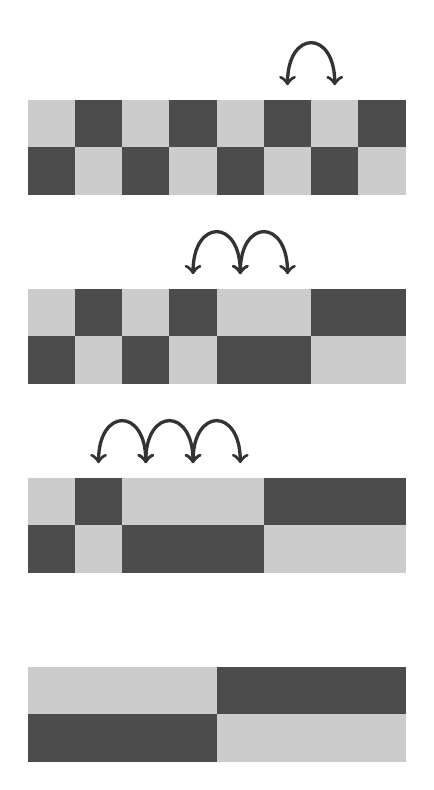
\begin{tikzpicture}[scale = 0.6]
\begin{scope}[shift = {(0,0)}]

    \fill[fill=black!20] (-2,0) rectangle (-1,1);
    \fill[fill=black!70] (-1,0) rectangle (0,1);
    \fill[fill=black!20] (0,0) rectangle (1,1);
    \fill[fill=black!70] (1,0) rectangle (2,1);
    \fill[fill=black!20] (2,0) rectangle (3,1);
    \fill[fill=black!70] (3,0) rectangle (4,1);
    \fill[fill=black!20] (4,0) rectangle (5,1);
    \fill[fill=black!70] (5,0) rectangle (6,1);
    
    \fill[fill=black!70] (-2,-1) rectangle (-1,0);
    \fill[fill=black!20] (-1,-1) rectangle (0,0);
    \fill[fill=black!70] (0,-1) rectangle (1,0);
    \fill[fill=black!20] (1,-1) rectangle (2,0);
    \fill[fill=black!70] (2,-1) rectangle (3,0);
    \fill[fill=black!20] (3,-1) rectangle (4,0);
    \fill[fill=black!70] (4,-1) rectangle (5,0);
    \fill[fill=black!20] (5,-1) rectangle (6,0);

     \draw[arrow_double] (3.5,1.2) .. controls (3.5, 2.5) and (4.5, 2.5) .. (4.5, 1.2);
\end{scope}

\begin{scope}[shift = {(0,-4)}]

    \fill[fill=black!20] (-2,0) rectangle (-1,1);
    \fill[fill=black!70] (-1,0) rectangle (0,1);
    \fill[fill=black!20] (0,0) rectangle (1,1);
    \fill[fill=black!70] (1,0) rectangle (2,1);
    \fill[fill=black!20] (2,0) rectangle (3,1);
    \fill[fill=black!20] (3,0) rectangle (4,1);
    \fill[fill=black!70] (4,0) rectangle (5,1);
    \fill[fill=black!70] (5,0) rectangle (6,1);
    
    \fill[fill=black!70] (-2,-1) rectangle (-1,0);
    \fill[fill=black!20] (-1,-1) rectangle (0,0);
    \fill[fill=black!70] (0,-1) rectangle (1,0);
    \fill[fill=black!20] (1,-1) rectangle (2,0);
    \fill[fill=black!70] (2,-1) rectangle (3,0);
    \fill[fill=black!70] (3,-1) rectangle (4,0);
    \fill[fill=black!20] (4,-1) rectangle (5,0);
    \fill[fill=black!20] (5,-1) rectangle (6,0);

    \draw[arrow_double] (1.5,1.2) .. controls (1.5, 2.5) and (2.5, 2.5) .. (2.5, 1.2);
    \draw[arrow_double] (2.5,1.2) .. controls (2.5, 2.5) and (3.5, 2.5) .. (3.5, 1.2);
\end{scope}

\begin{scope}[shift = {(0,-8)}]

    \fill[fill=black!20] (-2,0) rectangle (-1,1);
    \fill[fill=black!70] (-1,0) rectangle (0,1);
    \fill[fill=black!20] (0,0) rectangle (1,1);
    \fill[fill=black!20] (1,0) rectangle (2,1);
    \fill[fill=black!20] (2,0) rectangle (3,1);
    \fill[fill=black!70] (3,0) rectangle (4,1);
    \fill[fill=black!70] (4,0) rectangle (5,1);
    \fill[fill=black!70] (5,0) rectangle (6,1);
    
    \fill[fill=black!70] (-2,-1) rectangle (-1,0);
    \fill[fill=black!20] (-1,-1) rectangle (0,0);
    \fill[fill=black!70] (0,-1) rectangle (1,0);
    \fill[fill=black!70] (1,-1) rectangle (2,0);
    \fill[fill=black!70] (2,-1) rectangle (3,0);
    \fill[fill=black!20] (3,-1) rectangle (4,0);
    \fill[fill=black!20] (4,-1) rectangle (5,0);
    \fill[fill=black!20] (5,-1) rectangle (6,0);

    \draw[arrow_double] (-0.5,1.2) .. controls (-0.5, 2.5) and (0.5, 2.5) .. (0.5, 1.2);
    \draw[arrow_double] (0.5,1.2) .. controls (0.5, 2.5) and (1.5, 2.5) .. (1.5, 1.2);
    \draw[arrow_double] (1.5,1.2) .. controls (1.5, 2.5) and (2.5, 2.5) .. (2.5, 1.2);
\end{scope}

\begin{scope}[shift = {(0,-12)}]

    \fill[fill=black!20] (-2,0) rectangle (-1,1);
    \fill[fill=black!20] (-1,0) rectangle (0,1);
    \fill[fill=black!20] (0,0) rectangle (1,1);
    \fill[fill=black!20] (1,0) rectangle (2,1);
    \fill[fill=black!70] (2,0) rectangle (3,1);
    \fill[fill=black!70] (3,0) rectangle (4,1);
    \fill[fill=black!70] (4,0) rectangle (5,1);
    \fill[fill=black!70] (5,0) rectangle (6,1);
    
    \fill[fill=black!70] (-2,-1) rectangle (-1,0);
    \fill[fill=black!70] (-1,-1) rectangle (0,0);
    \fill[fill=black!70] (0,-1) rectangle (1,0);
    \fill[fill=black!70] (1,-1) rectangle (2,0);
    \fill[fill=black!20] (2,-1) rectangle (3,0);
    \fill[fill=black!20] (3,-1) rectangle (4,0);
    \fill[fill=black!20] (4,-1) rectangle (5,0);
    \fill[fill=black!20] (5,-1) rectangle (6,0);

\end{scope}[shift = {(-2,0)}]

\end{tikzpicture}
\end{figure}


\end{document}